

\tikzset{every picture/.style={line width=0.75pt}} %set default line width to 0.75pt        

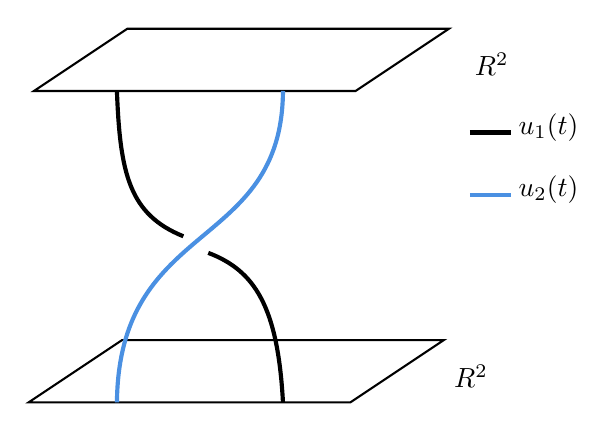
\begin{tikzpicture}[x=0.75pt,y=0.75pt,yscale=-1,xscale=1]
%uncomment if require: \path (0,877); %set diagram left start at 0, and has height of 877

%Shape: Rectangle [id:dp23975536104774442] 
\draw   (205,60) -- (360,60) -- (315,90) -- (160,90) -- cycle ;
%Shape: Rectangle [id:dp4742593007559085] 
\draw   (202.5,210) -- (357.5,210) -- (312.5,240) -- (157.5,240) -- cycle ;
%Straight Lines [id:da17288821057020853] 
\draw [line width=1.5]    (370,110) -- (390,110) ;
%Straight Lines [id:da7810709935908421] 
\draw [color={rgb, 255:red, 74; green, 144; blue, 226 }  ,draw opacity=1 ][line width=1.5]    (370,140) -- (390,140) ;
%Curve Lines [id:da18292473776224472] 
\draw [color={rgb, 255:red, 74; green, 144; blue, 226 }  ,draw opacity=1 ][line width=1.5]    (280,90) .. controls (279.5,168) and (201,151) .. (200,240) ;
%Curve Lines [id:da8202799075901603] 
\draw [line width=1.5]    (200,90) .. controls (201.5,130) and (206,149.5) .. (232,160) ;
%Curve Lines [id:da7930766509930773] 
\draw [line width=1.5]    (244,168) .. controls (266.5,176.5) and (277.5,194) .. (280,240) ;

% Text Node
\draw (371,70.4) node [anchor=north west][inner sep=0.75pt]    {$\mathbb{R}^{2}$};
% Text Node
\draw (361,220.4) node [anchor=north west][inner sep=0.75pt]    {$\mathbb{R}^{2}$};
% Text Node
\draw (392,99.4) node [anchor=north west][inner sep=0.75pt]    {$u_{1}( t)$};
% Text Node
\draw (392,129.4) node [anchor=north west][inner sep=0.75pt]    {$u_{2}( t)$};


\end{tikzpicture}
